\section{Non-Standard Interactions}\label{sec:nsiTheory}
We have no reason to believe that the Standard Model 
gauge group is the complete picture. We have already seen how the failure of the Standard Model to predict neutrino masses and 
oscillations forces us to amend it. 
Just as the electroweak theory $SU(2)_L \times U(1)_Y$ is 
spontaneously broken to $U(1)_{EM}$, a higher order theory at a different energy scale with completely different
properties might undergo a similar spontaneous symmetry break at high energies, 
producing at lower energies the Standard Model that we know. In fact, 
just as the fermion masses originate from the electroweak symmetry breaking, the neutrino masses might be generated from 
another broken symmetry resulting in the Standard Model gauge group.
In this sense, the Standard Model might be considered 
an effective low energy theory, which is yields impressive results in some areas, but failing in others. 

Compared to other fermions, the lightness of neutrino masses\footnote{The extreme lightness might be explained by a mass generation at a higher order theory.} along with their sparse SM interactions might 
indicate that these particles provide the best starting point for us to probe new physics, in which exotic neutrino interactions might occur~\cite{gavela2009}. We call these interactions non-standard interactions (NSI) in order to 
distinguish them from the `standard' interactions of the Standard Model.
 
Following the approach of the Standard Model that the group generators uniquely determine the gauge bosons, a different gauge
theory will have different interactions than those we presently know. These new interactions can be parametrized as model-independent four-fermion effective operators \cite{salvadoNSI,nsiFarzan}.
Following the discussion in~\cite{tommyNSI}, we see that the NSI parameters $\epsilon$ resulting from six-dimensional operators have the scale
\begin{align}
    \epsilon \propto \frac{m_W^2}{m_{\epsilon}^2} \sim \frac{10^{-2}}{m_\epsilon^2}\,
\end{align} 
in \si{\TeV}, so the new interactions generated at a mass scale of $m_\epsilon = \SI{1}{TeV}$ will produce parameters in the order of $10^{-2}$, 
two magnitudes below the standard matter effect. Thus, if we assume the new interactions to arise from a higher-energy theory above electroweak scale, 
we then predict that the parameters contribute with at most a factor of $10^{-2}$ to the standard matter effect, decreasing quadratically.


\subsection{Non-Standard Effects on Neutrino Matter Interactions}
Up until now, we have only considered weak neutrino interactions with electrons, protons, and neutrons.
We can phenomenologically allow these interactions to include the up and down quarks which are present 
in the Earth as the fundamental components of neutrons and protons, as seen in the Lagrangians
\begin{align*}
    \mathcal{L}_{\mathrm{CC}} &= -2 \sqrt{2} G_{F} \epsilon_{\alpha \beta}^{f f^{\prime} X}\left(\bar{\nu}_{\alpha} \gamma^{\mu} P_{L} \ell_{\beta}\right)\left(\bar{f}^{\prime} \gamma_{\mu} P_{X} f\right) \\
    \mathcal{L}_{\mathrm{NC}} &= -2 \sqrt{2} G_{F} \epsilon_{\alpha \beta}^{f X}\left(\bar{\nu}_{\alpha} \gamma^{\mu} P_{L} \nu_{\beta}\right)\left(\bar{f} \gamma_{\mu} P_{X} f\right)\,,
\end{align*}
where CC denotes the charged current interaction with the matter field $f\neq f^\prime \in \{u,d\}$, and NC denotes the neutral current interaction with 
$f \in \{e,u,d\}$. The CC NSI effect affects neutrino production and detection, and will not be considered further. NC NSI affect the matter potential, 
and is thus of interest to us.

We have no independent sensitivity for the neither chirality nor flavor type of $\epsilon^X$, so we sum over these and study the effective matter NSI parameter
 $\epsilon_{\ab}$:
\begin{align}
    \epsilon_{\ab} = \sum_{X \in \{L,R\}} \sum_{f \in \{e,u,d\}} \frac{N_f}{N_e} \epsilon^{fX}_{\ab}\,.
\end{align}
Our matter study will be wholly confined to the interior of the Earth, where we assume electrical neutrality and equal distribution of neutrons and protons, 
we get $N_u/N_e \simeq N_d/N_e \simeq 3$. Also we assume the components $\epsilon_{\a\b}$ to be real. Thus,
\begin{align}
    \epsilon_{\ab} =  \sum_X \epsilon_{\ab}^{eX} + 3(\epsilon_{\ab}^{uX} + \epsilon_{\ab}^{dX})
\end{align}
Now, $\epsilon_{\ab}$ enters the Hamiltonian as entries of a potential-like matrix. In Eq.~\ref{eq:NSIH}, $A_{CC}\text{diag}(1,0,0)$ is our 
familiar matter potential from the Standard Model. There is also our new term, $A_{CC} \epsilon$, which contains the components $\epsilon_{\a\b}$:
\begin{align}\label{eq:NSIH}
    H &= \frac{1}{2E} \left[UM^2U^\dagger + A_{CC}\,\text{diag}(1,0,0) + A_{CC}\, \epsilon \right] \nonumber \\
      &= \frac{1}{2E} \left[UM^2U^\dagger + A_{CC}
      \begin{pmatrix}
          1 + \epsilon_{ee} & \epsilon_{e\mu} & \epsilon_{e\tau}  \\
          \epsilon_{\mu e} & \epsilon_{\mu\mu} & \epsilon_{\mu\tau}  \\
          \epsilon_{\tau e} & \epsilon_{\tau\mu} & \epsilon_{\tau\tau}
      \end{pmatrix} \right]\,.
\end{align} 
In the limit $\epsilon_{\ab} \to 0$, we recover the standard interaction Hamiltonian from Eq.~\ref{eq:H_3gen}.
We can draw several conclusions from this form of the Hamiltonian. Any nonzero off-diagonal element $\epsilon_{\ab}, \a \neq \b$ contribute
to neutrino mixing, just as the off-diagonal elements of $U$ does in the SM. Moreover, since the SM potential has the same order in $A_{CC}$ as the NSIs, 
any $\epsilon_{\ab} \sim 1$ will make the new matter effect be the same order as the SM effect.

We have two more modifications to the matrix $\epsilon$. First, all terms of the Hamiltonian must of course be Hermitian, thus
\begin{align}
    \begin{pmatrix}
        \epsilon_{ee} & \epsilon_{e\mu} & \epsilon_{e\tau}  \\
        \epsilon_{\mu e} & \epsilon_{\mu\mu} & \epsilon_{\mu\tau}  \\
        \epsilon_{\tau e} & \epsilon_{\tau\mu} & \epsilon_{\tau\tau}
    \end{pmatrix} =
    \begin{pmatrix}
        \epsilon_{ee} & \epsilon_{e\mu} & \epsilon_{e\tau}  \\
        \epsilon_{e \mu} & \epsilon_{\mu\mu} & \epsilon_{\mu\tau}  \\
        \epsilon_{e\tau} & \epsilon_{\mu\tau} & \epsilon_{\tau\tau}
    \end{pmatrix}\,.
\end{align}
Now we have reduced the possible number of NSI parameters from 9 down to 6. 

By combining oscillation data and neutrino-nucleon scattering at the COHERENT experiment, 90 \% CL ranges of some of 
the NSI parameters were constrained in~\cite{coherent} to
\begin{align}\label{eq:coherentbounds}
    -0.090 < &\,\ett < 0.38 \nonumber \\
    -0.01 < &\,\emt < 0.009 \nonumber \\
    -0.073 < &\,\eem < 0.044 \nonumber \\
    -0.15 < &\,\eet < 0.13\,.
\end{align}


\subsection{IceCube Signal}
In our analysis of IceCube, we are constrained to muon track events. Thus, we are not able to test any theory which does not modify $P_{\a \mu}$. Moreover,
the IceCube data is available in the range \SI{500}{\GeV} to \SI{10}{\TeV} range, where any rapid oscillations have averaged out.

Since all standard matter potentials are diagonal, 
the elements $\epsilon_{\a\b},\, \a = \b$ will directly adjust the matter potential felt 
by flavor $\a$. The off-diagonal terms have a more interesting theoretical implication as they open up matter interactions across flavors. Remember, in the Standard model,
we are restricted to weak interactions that conserve lepton flavor. However, an off-diagonal NSI parameter allows flavor transitions during matter interactions. Thus,
the off-diagonal elements constitute new sources of flavor violation.
Moreover, $\epsilon_{\a\b}$ modifies the $\nu_\a \to \nu_\b$ transition independently
of the mixing matrix. Thus, we are not confined to the parameters of the mixing matrix: now we have introduced the 
possibility of additional interactions that can cause the flavor change. Moreover, since we have 6 NSI parameters, and the PMNS
matrix is parametrized with only 3 parameters, we have more degrees of freedom when adjusting the probabilities using the NSI matrix. Each term in the PMNS matrix consists of at least
two of the three mixing angles, making the individual angles more inter-dependent than the NSI parameters, since combinations of them must satisfy the constraints of the matrix elements.

As discussed in Eq.~\ref{eq:Uvalues}, the atmospheric $\nm \to \nt$ transition will be the most abundant, making $\emt$, $\emm$, $\ett$ the most suitable
NSI parameters to constrain from muon events. As we will see, $\eem$ is also a candidate, albeit a weaker one. 

In Fig.~\ref{fig:emt_ett_probs}, we see how the introduction of $\emt = 0.02$ alters the $\nm$ and $\anm$ survival probabilities
for neutrinos that traverse the entire Earth diameter (i.e. $\ztrue = -1$). $\emt$ does not dramatically change neither
amplitude nor frequency of the probabilities. Instead, it seems to stretch or compress the oscillations. Since the 
only difference between the way neutrinos and antineutrinos interact with matter is the sign of the potential, the probability for
$\nm$ with positive $\epsilon_{\a\b}$ is identical to the probability for $\anm$ with negative $\epsilon_{\a\b}$. Thus, the dashed line 
in the right panel not only shows the survival probability for $\anm$ with $\emt=0.02$, but also the survival probability for $\nm$ with $\emt=-0.02$.
Hence, we note that $\emt > 0$ stretches (compresses) $\Pmm$ for neutrinos (antineutrinos), while $\emt < 0$ compresses (stretches) $\Pmm$ for neutrinos (antineutrinos).

The value of $\ett$ affects neither $\Pmm$ nor $\Pamam$, in the IceCube region above \SI{500}{\GeV}. Hence, we will not be able
to say anything about $\ett$ in our IceCube study.  Comparing the probabilities in Fig.~\ref{fig:emt_ett_probs} with $\ett = 0.05$ with the ones for $\emt = 0.02$ in Fig.~\ref{fig:emt_ett_probs},
we see that even though we let $\ett$ take 2.5 times the value of $\emt$, its effect on $\Pmm$ is smaller. The weakening of the $\Pamam$ resonance will be visible in DeepCore, but we should expect a less stringent 
constraint due to the weakness of the effect compared to $\emt$. 

Thus, we will use IceCube to constrain $\emt$ only.


Moving on to $\eem$ and Fig.~\ref{fig:eem_eet_probs}, we see that both probabilities has shifted downwards for $\Etrue > \SI{500}{\GeV}$.
In Fig.~\ref{fig:eem_eet_probs}, we see that the muon channel remains largely unaffected of the value of $\eet$ as we expected. The exception of this lies 
in the DeepCore region of rapid oscillations, where mixing is more violent. 
\begin{figure}
    \begin{center}
        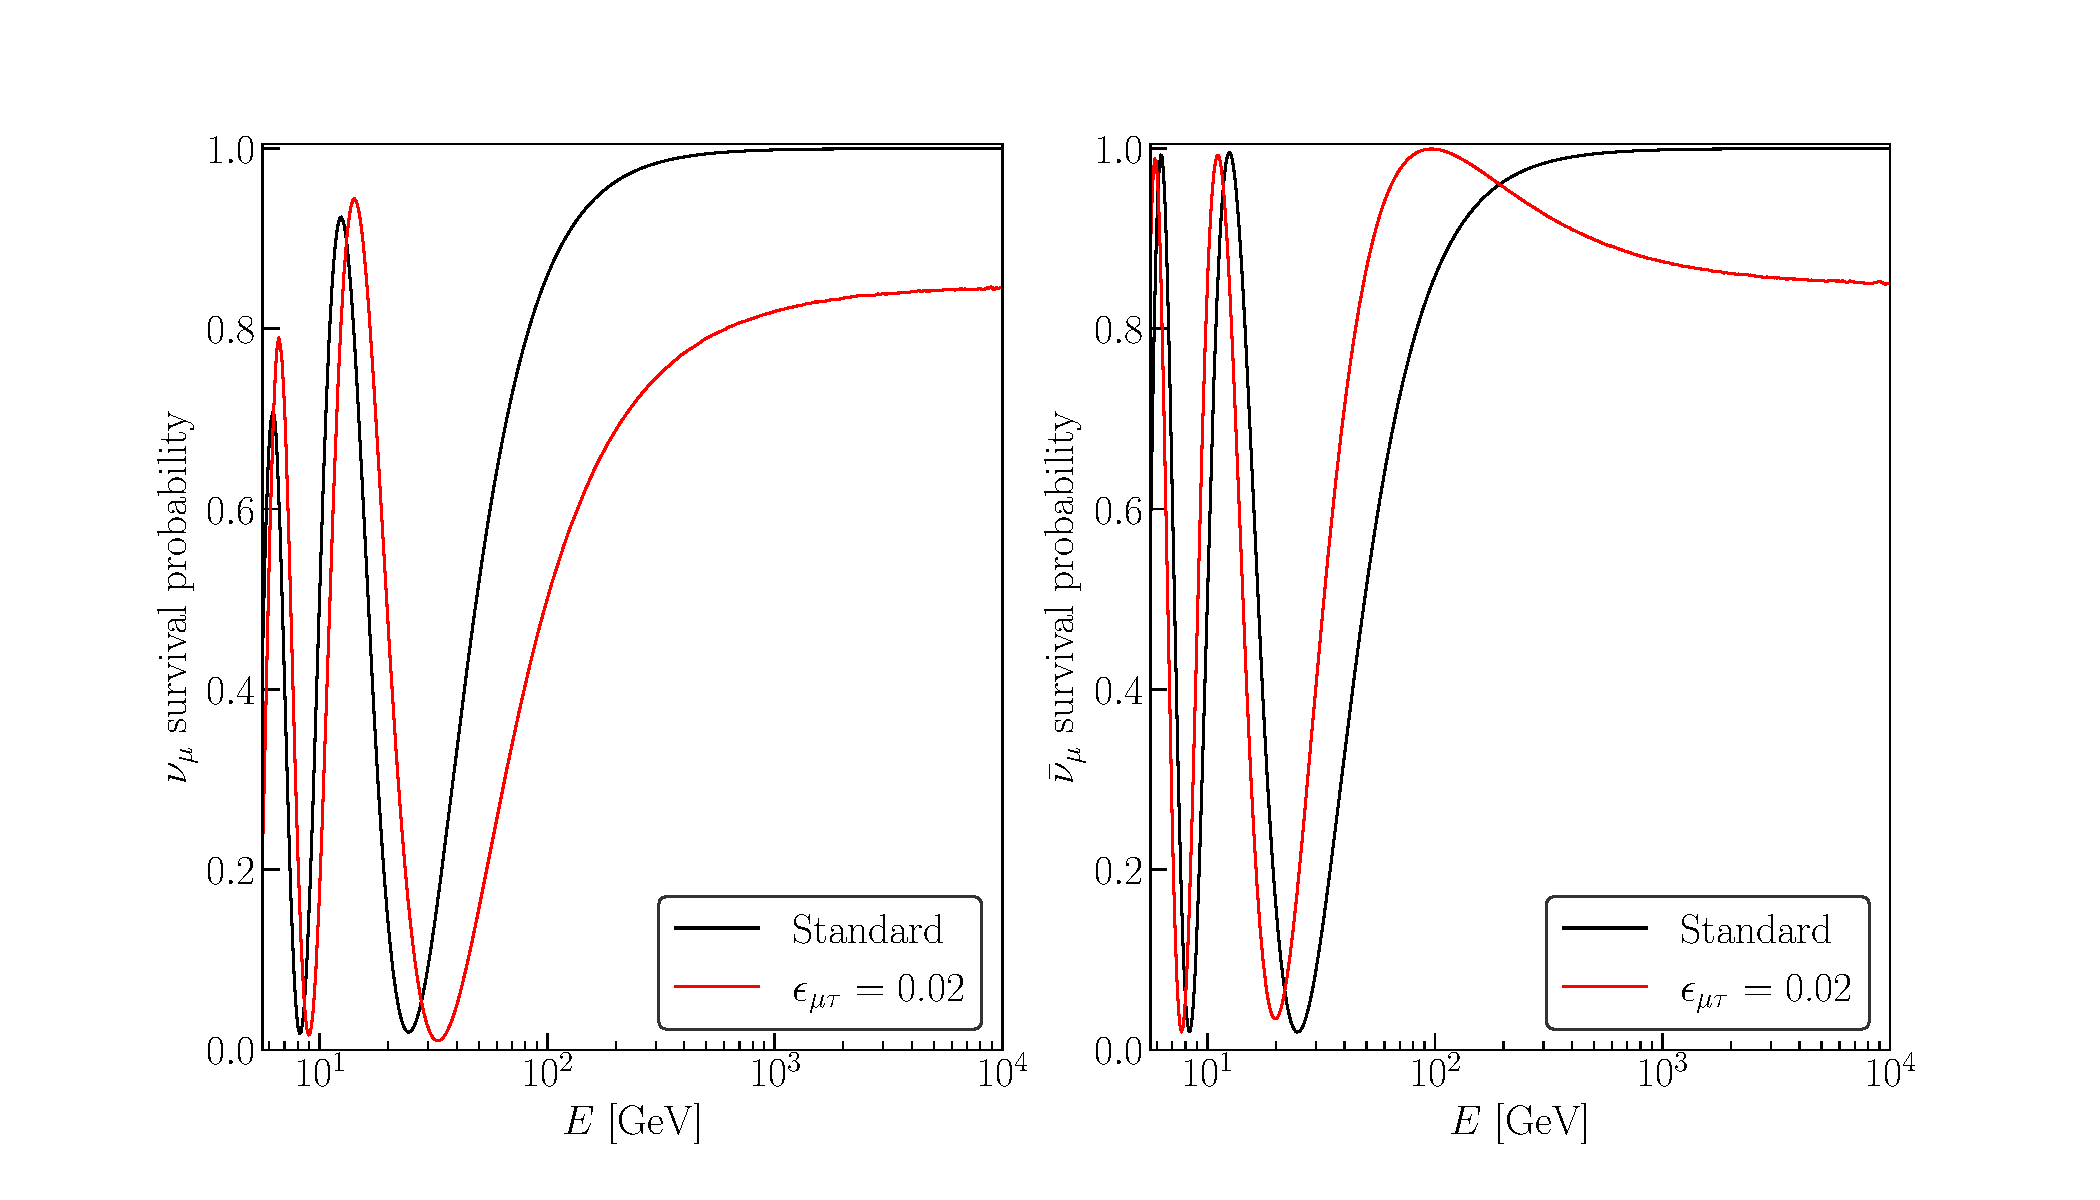
\includegraphics[width=0.99\textwidth]{figures/Pmm_emt_probs.pdf}
        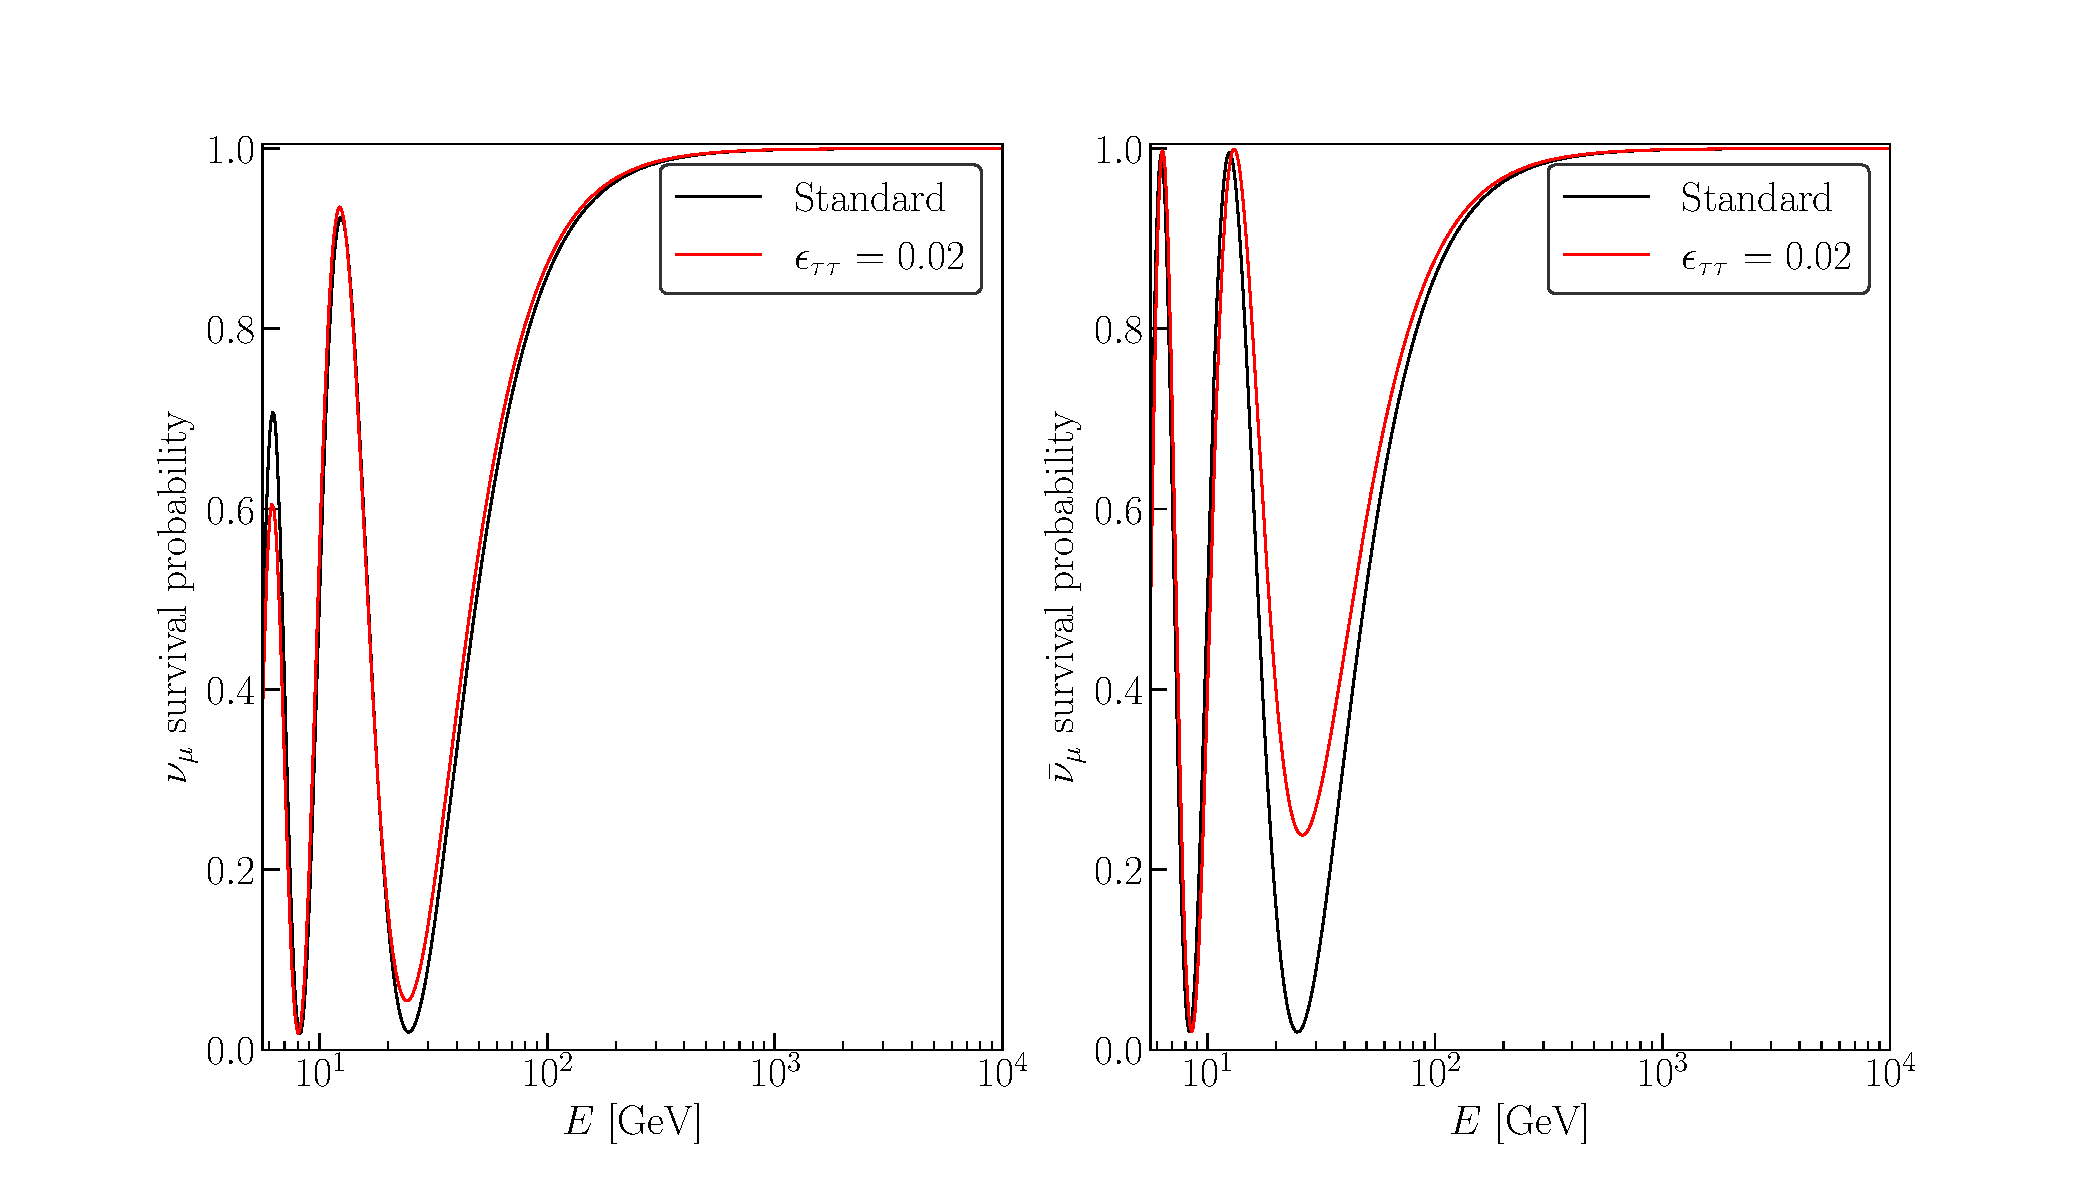
\includegraphics[width=0.99\textwidth]{figures/Pmm_ett_probs.pdf}
        \caption{\emph{Top panel:} Muon neutrino and antineutrino survival probabilities for
        $\ztrue = -1$ when $\emt = 0.02$. All other NSI parameters are fixed to zero. In the \si{\GeV} range, $\emt$ shifts the oscillations to the right for $\nm$, and to the left for $\anm$. At \si{\TeV} energies, both probabilities simply get shifted down, resulting in a net reduction of track events.
        \emph{Bottom panel:} Muon neutrino and antineutrino survival probabilities for
        $\ztrue = -1$ when $\ett = 0.05$. All other NSI parameters are fixed to zero. $\ett$ does not affect the probabilities above \SI{100}{\GeV} and this parameter is thus unable to be constrained by tracks in IceCube in our study. However, the dampening of the $\anm$ survival probability will be visible to DeepCore and PINGU, since it occurs within their energy ranges.}
        \label{fig:emt_ett_probs}
    \end{center}
\end{figure}


\begin{figure}
    \begin{center}
        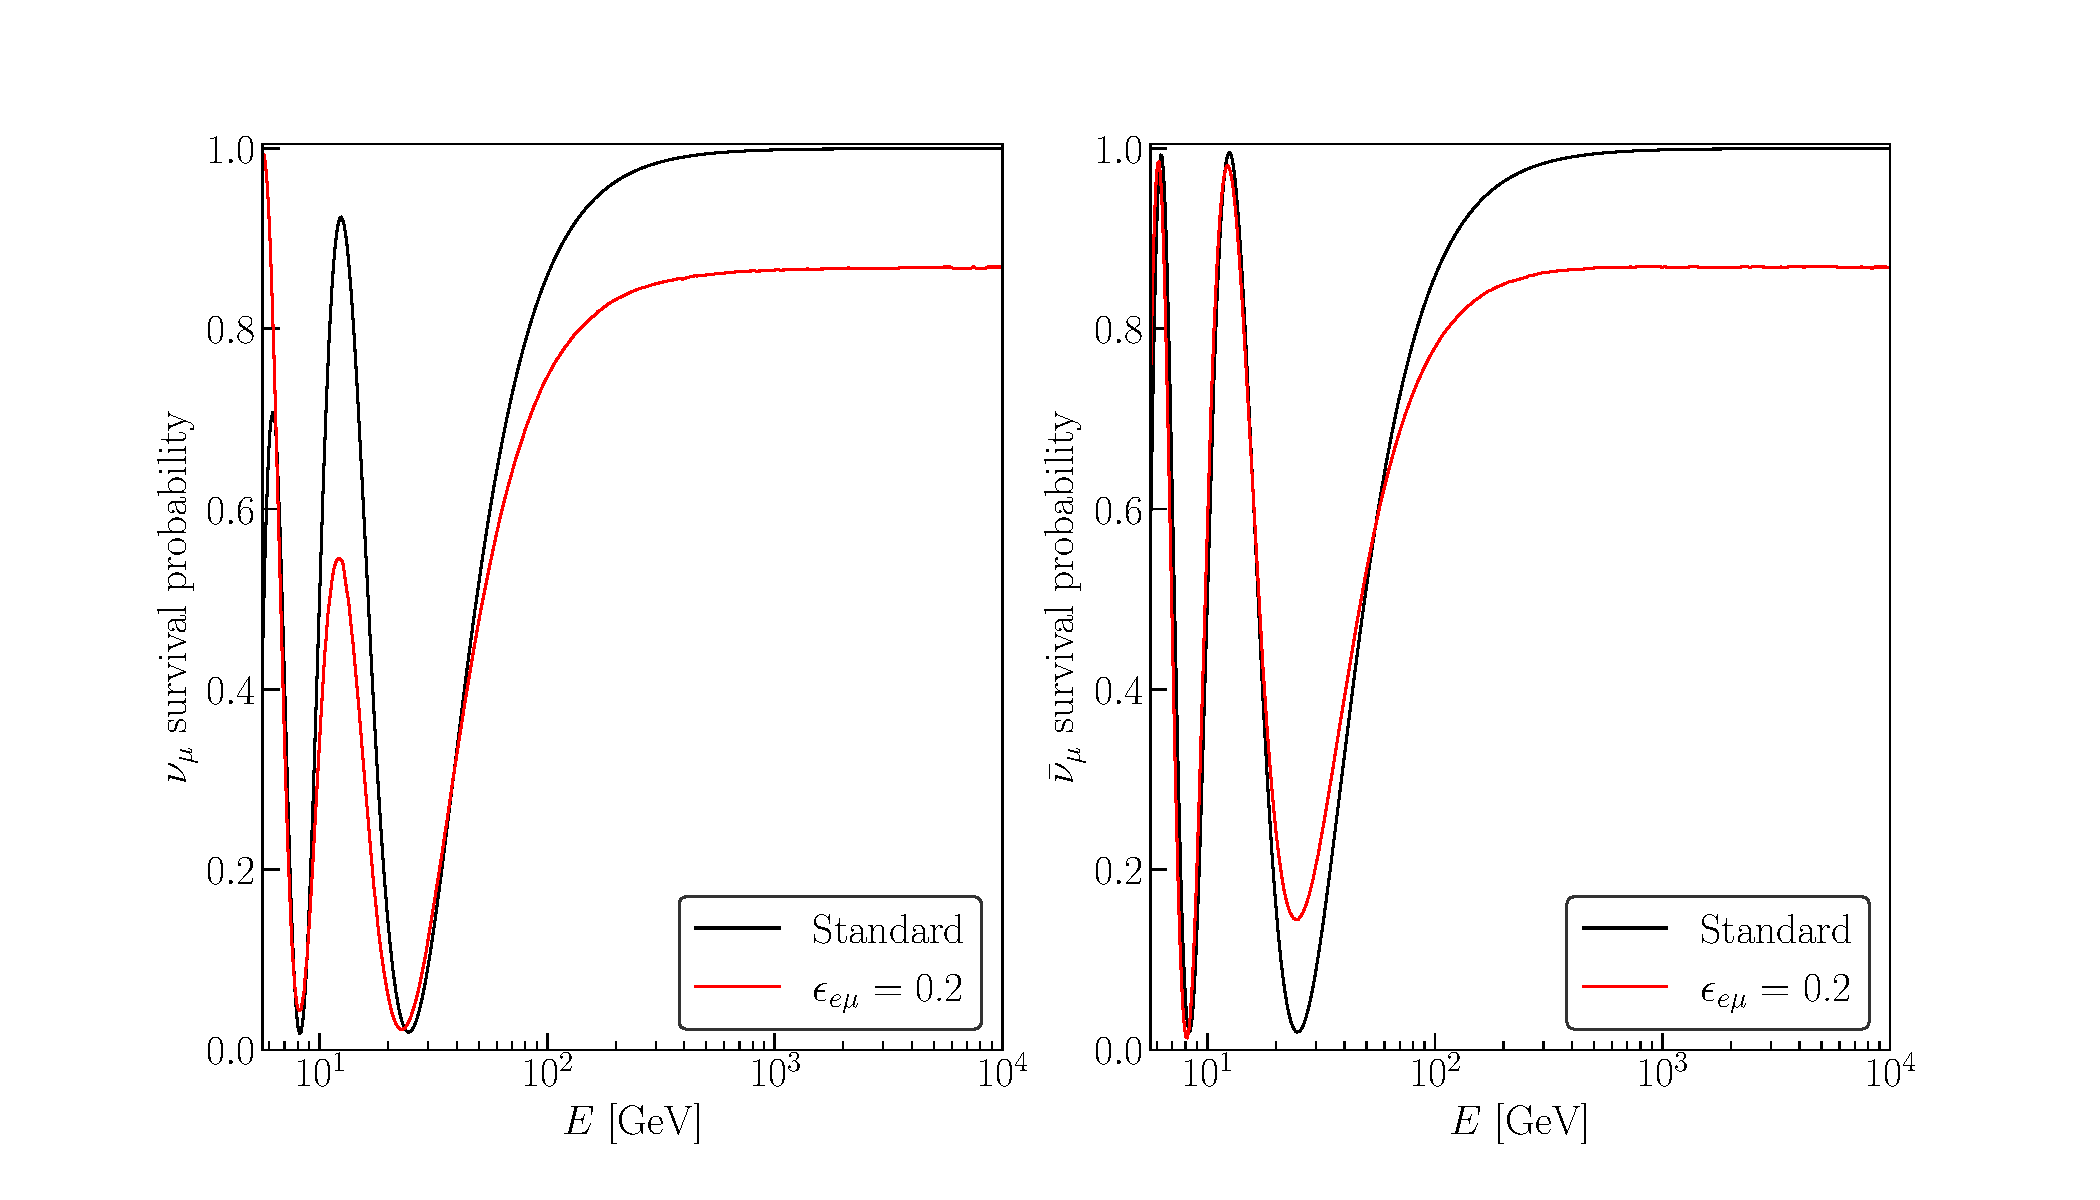
\includegraphics[width=0.99\textwidth]{figures/eem_probs.pdf}
        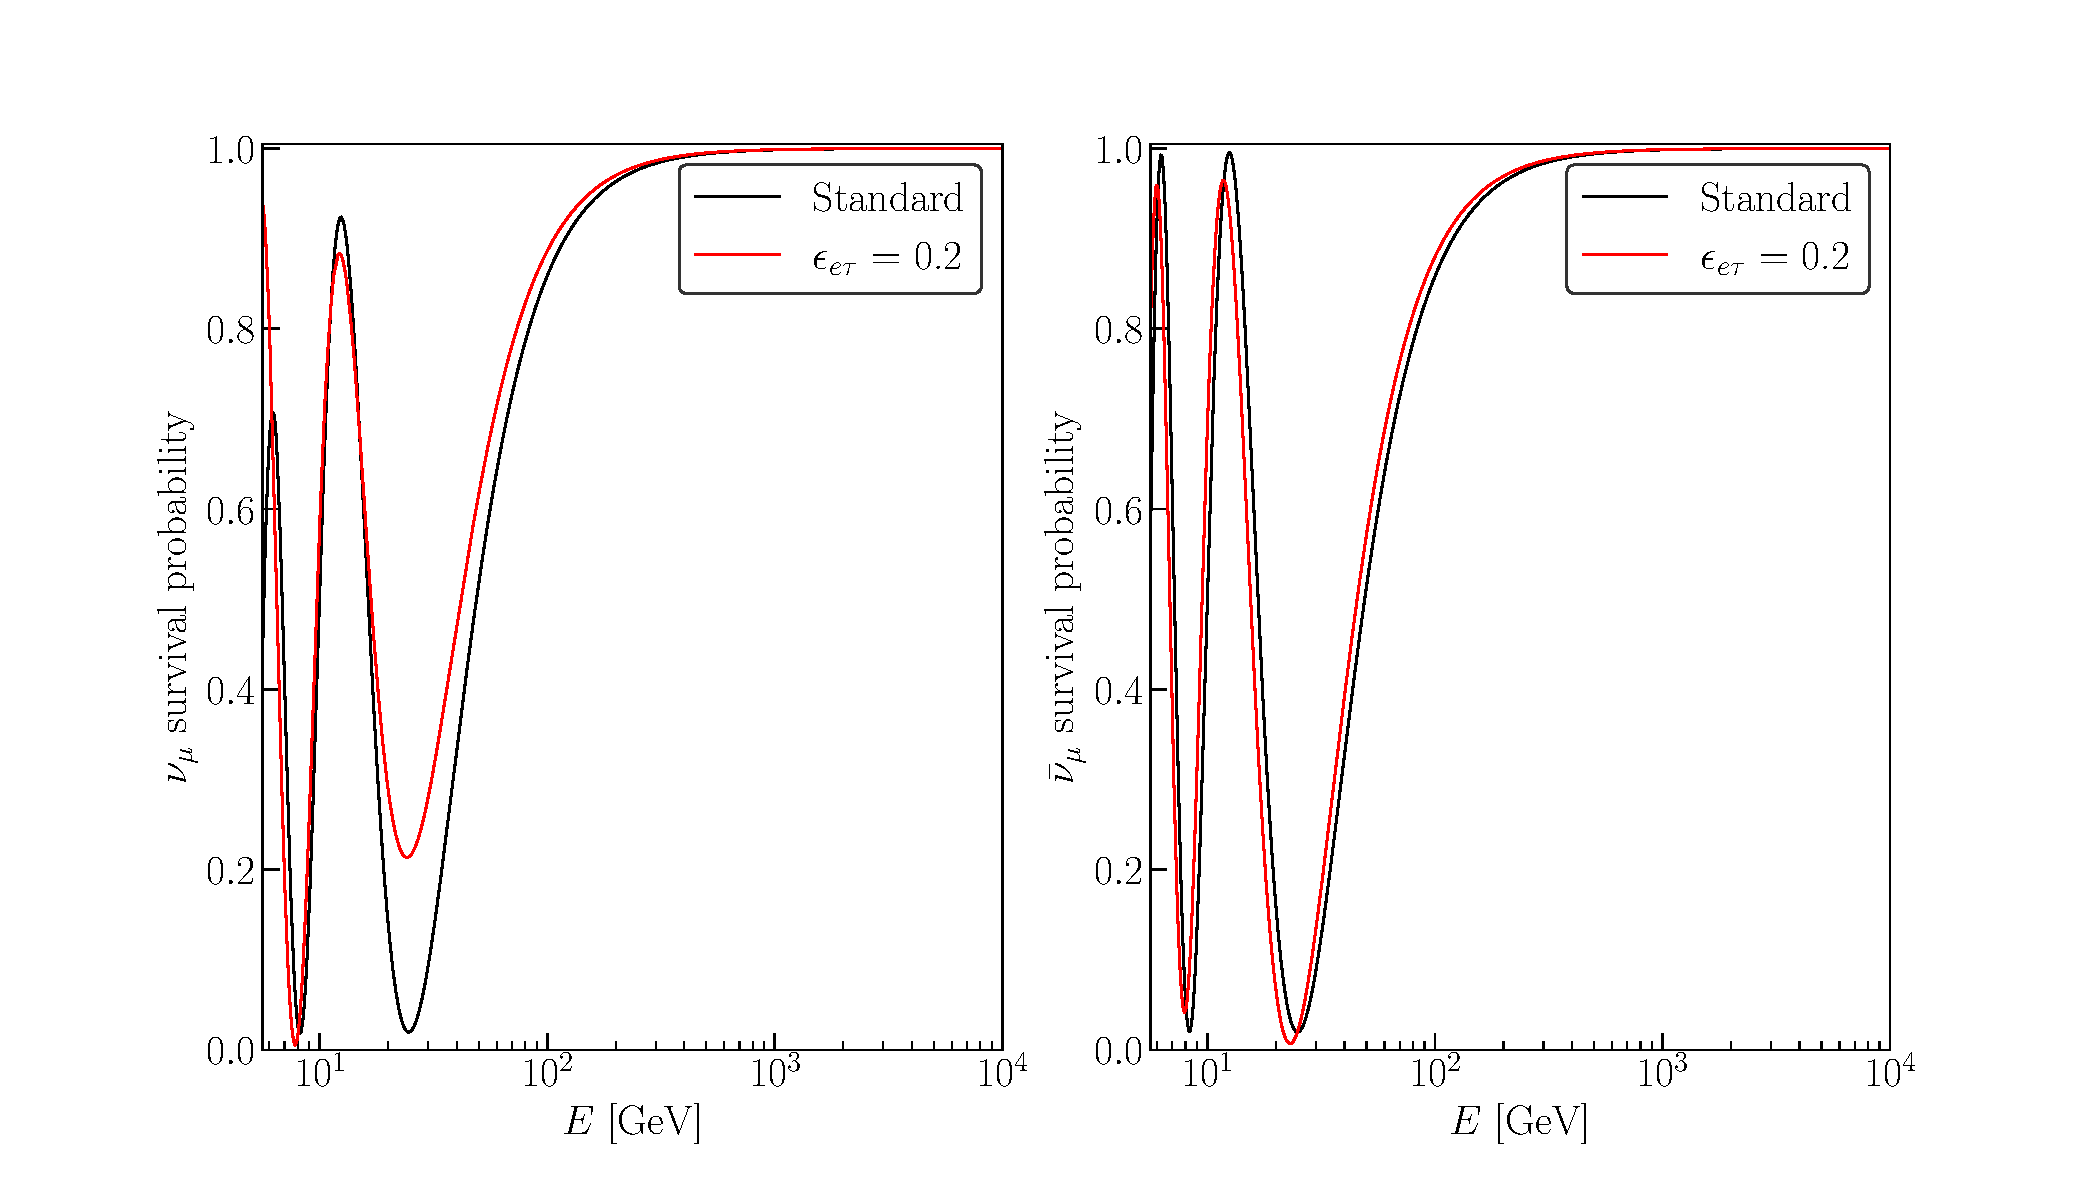
\includegraphics[width=0.99\textwidth]{figures/eet_probs.pdf}
        \caption{Muon neutrino and antineutrino survival probabilities for
        $\ztrue = -1$. \emph{Top panel:} $\eem = 0.2$. All other NSI parameters are fixed to zero. Instead of the oscillations shifting to the left or right, $\eem$ dampens an oscillation peak for low \si{\GeV}. At \si{\TeV}, the probability is shifted down, just as with $\emt$.
        \emph{Bottom panel:} $\eet = 0.2$. All other NSI parameters are fixed to zero. Here, we see a very weak shifting and a $\nm$ weaker dip at low \si{\GeV}, and again, no visible effect at \si{TeV} energies. }
        \label{fig:eem_eet_probs}
    \end{center}
\end{figure}


\subsection{DeepCore and PINGU Signals}
Now we repeat our probability analysis but for the DeepCore/PINGU region of \SIrange{5.6}{56}{\GeV}. As we previously saw,
we have rapid oscillations, which means that `indirect' modifications (i.e. $\eet$ will affect the $\Pmm$ channel)
will be more apparent, since all flavors are involved to a greater degree compared with the more stable region above \SI{500}{\GeV}, where 
many oscillations have averaged out.

Another feature of our DeepCore study includes the fact that we now have access to cascade events, in which $\ne$ and $\nt$ are more abundant.
Thus, we are no longer constrained to the $\mu$ channel alone, but we can now find interesting features in the other channels too. However, we 
remember that the $\nm$ flux is still the most abundant.

Fig.~\ref{fig:emt_ett_probs} shows that $\emt$ affects both $\Pmm$ and $\Pamam$ over the whole energy range. Since 
IceCube also sees this, we hope to be able to boost the constraining of $\emt$ by combining the two experiments.

Regarding $\ett$ in Fig.~\ref{fig:eem_eet_probs}, the signal mainly shows in the $\Pamam$ channel as
a shallower dip in the \SI{20}{\GeV} region. Thus, DeepCore/PINGU alone will be used to constrain this parameter.

$\eem$ in Fig.~\ref{fig:eem_eet_probs} causes a weaker dip for both $\nm$ and $\anm$. 

For $\eet$, we see a similar effect on the dip in $\Pmm$ as we did with $\ett$ for $\Pamam$. Hence, we should be able to 
see the $\eet$ effect in DeepCore/PINGU. Remember that we now have the option to look at the other flavor channels than $\mu$ since we 
have cascade events for DeepCore and PINGU. If we simulate 
$\Pme^{NSI}$ at three different energies, and let both $\eem$ and $\eet$ vary together between the values $\{-0.3,0.3\}$, we produce a two-dimensional grid of probabilities.
Subtract the regular $\Pme^{SI}$ (that is, no NSI), and take the absolute value of the difference. We see the result in Fig.~\ref{fig:eem_eet_prob}. 
The middle and right panels, which show the absolute probability difference at \si{25} and $\SI{50}{\GeV}$, respectively, are very bleak,
indicating that the impact of the NSI parameters $\eem$ and $\eet$ is not as strong at these energy levels. Turning to the left-most panel,
we see a region in which the difference again is close to zero, but now surrounded by fringes of very large differences, up to $50\%$ difference 
in the $\Pme$ probability. This indicating that the NSI parameters are much more influential at these energies, and that we should be able to 
constrain both $\eem$ and $\eet$ from $\SI{5}{\GeV}$ cascade events.

\begin{figure}
    \centering
    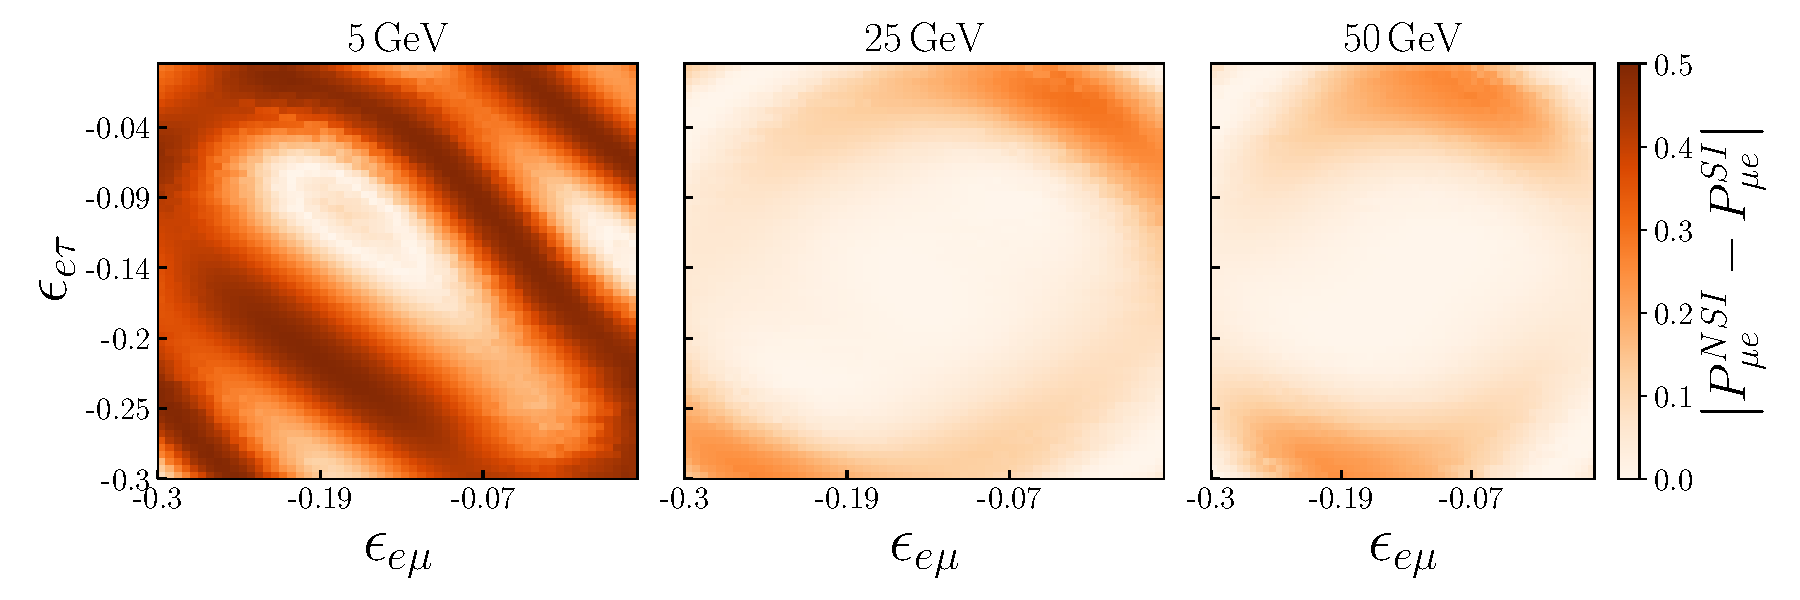
\includegraphics[width=1\textwidth]{figures/eem_eet_prob.pdf}
    \caption{The quantity $\abs{P_{\mu e}^{NSI} - P_{\mu e}^{SI}}$ when we let $\eem$ and $\eet$ independently vary over
    the range \{-0.3,0.3\} at \si{5}, \si{25}, and $\SI{50}{\GeV}$. At $\SI{5}{\GeV}$, we see strong deviations in the probabilities, showing
    a promising indication that constriction of $\eem$ and $\eet$ is possible using cascade events at these energies.}\label{fig:eem_eet_prob}
\end{figure}

Fig.~\ref{fig:Pee_eet_probs} shows the electron neutrino and antineutrino survival probabilities, and here we see
a clear difference when turning on $\eet$. 



\begin{figure}
    \begin{center}
        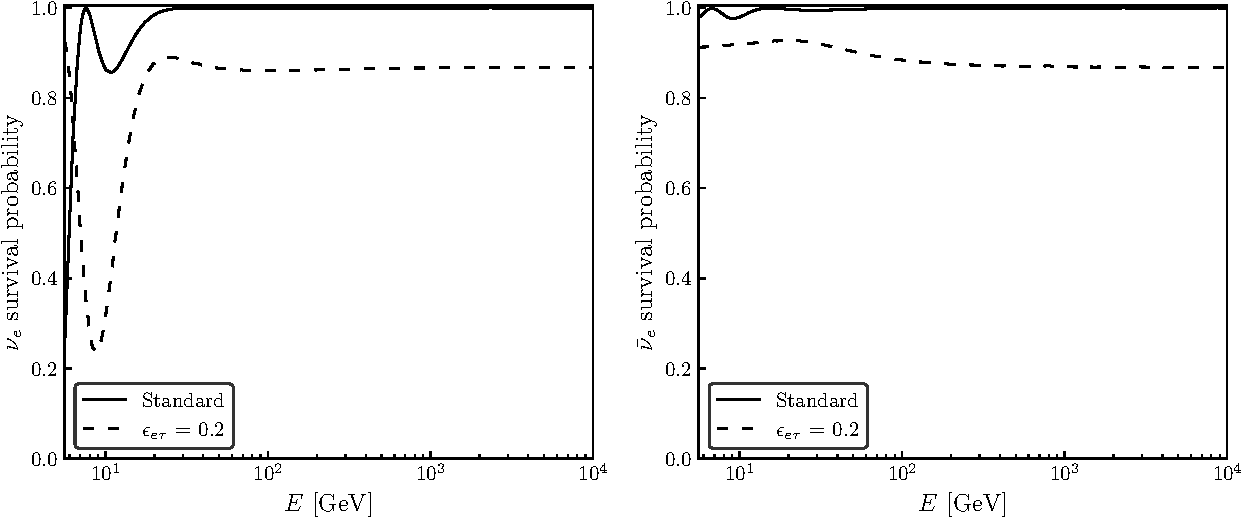
\includegraphics[width=0.9\textwidth]{figures/Pee_eet_probs.pdf}
        \caption{Electron neutrino and antineutrino survival probabilities for
        $\ztrue = -1$ when $\eet = 0.2$. All other NSI parameters are fixed to zero. Compared to the $\nm$ and $\anm$ plots, here we see a strong difference across the whole energy range.}
        \label{fig:Pee_eet_probs}
    \end{center}
\end{figure}
